\begin{document}

\def\title{Worksheet 2}

\newcommand{\qitem}{\qpart\item}

\renewcommand{\labelenumi}{(\alph{enumi})} % change default enum format to (a)
\renewcommand{\theenumi}{(\alph{enumi})} % fix reference format accordingly.
\renewcommand{\labelenumii}{\roman{enumii}.} % second level labels.
\renewcommand{\theenumii}{\roman{enumii}.}

\maketitle

\vspace{0.5em}

\begin{qunlist}



% Author: Yannan Tuo, Varsha Ramakrishnan, Taejin Hwang
% Email: ytuo@berkeley.edu, vio@berkeley.edu, taejin@berkeley.edu
% Edited Lydia Lee, Spring 2019
% lydia.lee@berkeley.edu
% Edited: Justin Yu, Spring 2020
% justinvyu@berkeley.edu

\qns{Eigendecomposition and Change of Basis}

\meta{
  Please do a mini-lecture on change of basis similar to the opening paragraph of the change of coordinates question before doing this one.It is crucial that students understand change of basis, and how to convert from different bases first, before trying to understand eigendecomposition. It is up to you whether you want to mention the fact that all diagonalizable linear operators have a diagonal matrix representation given the correct choice of basis.
}

\textbf{Diagonal matrices}, matrices where all entries outside of the diagonal are zero, are often desirable since they are easy to analyze.
Determining properties such as rank and invertibility, are much simpler on a diagonal matrix as opposed to other non-diagonal matrices.
The process of \textbf{changing to a basis} in which the linear operator has a diagonal matrix representation is called \textbf{eigendecomposition} or \textbf{diagonalization.} You can think of eigendecomposition as a change of basis to one entirely made up of eigenvectors.

So what is a \textbf{change of basis}? Consider an arbitrary vector in $\mathbb{R}^2$: $\vec{x} = [ x_1 \text{ } x_2 ]^T$.
When we write a vector in this form, we are representing it as a linear combination of the \textit{standard basis} vectors for $\mathbb{R}^2$: $\vec{x} = x_1 \begin{bsmallmatrix} 1 \\ 0 \end{bsmallmatrix} + x_2 \begin{bsmallmatrix} 0 \\ 1 \end{bsmallmatrix}$. Naturally, $x_1$ and $x_2$ are the \textit{coordinates} of $\vec{x}$ in the standard basis (as you would refer to them if you graphed $\vec{x}$ on a Cartesian plane).

Now what if we wanted to represent that same vector in a different basis?
For example, say you wanted to represent the same vector $\vec{x}$ using the set of basis vectors $\vec{v_1}$ and $\vec{v_2}$.
This means that we need to find scalars $\alpha_1$ and $\alpha_2$ such that $\vec{x}$ can be written as a linear combination of these new basis vectors: $\vec{x} = \alpha_1 \vec{v_1} + \alpha_2 \vec{v_2}$.
To do this, we can just setup and solve a system of linear equations of the form:
$$\begin{bmatrix} \vec{v_1} & \vec{v_2} \end{bmatrix} \begin{bmatrix} \alpha_1 \\ \alpha_2 \end{bmatrix} = \begin{bmatrix} x_1 \\ x_2 \end{bmatrix}$$

In this problem, we'll investigate changing to and from the \textbf{eigenbasis} for the following matrix:

$$A = \begin{bmatrix}
2 & 2 \\
5 & -1
\end{bmatrix}$$

\begin{enumerate}

\qitem \textbf{Find $\lambda_1, \lambda_2$, the eigenvalues of $A$, ordered from largest to smallest.}
\ws{
\vspace{200px}
}

\meta {
  These first two parts are optional if students are comfortable with the process of finding eigenvalues and eigenspaces.
  It gives some concrete values that students can try out for the rest of the problem. If your students aren't convinced
  by $A = VDV^{-1}$, have them try out the concrete example with the numbers calculated in the first two parts.
}

\sol{
  \begin{align*}
    \text{det}(A - \lambda I) &= 0 \\
    (2 - \lambda) (-1 - \lambda) - 2(5) &= 0 \\
    \lambda^2 - \lambda - 12 &= 0 \\
    \implies \lambda_1 &= 4 \\
    \lambda_2 &= -3
  \end{align*}
}

\qitem \textbf{Find the eigenvectors $\vec{v_1}, \vec{v_2}$ corresponding to the eigenvalues.}

\ws{
\vspace{200px}
}

\sol{
  % \begin{bmatrix} 1 \\ 1 \end{bmatrix} \\ \begin{bmatrix} 1 \\ -1 \end{bmatrix}
  $$\vec{v_1} = \alpha \begin{bmatrix} 1 \\ 1 \end{bmatrix}$$
  $$\vec{v_2} = \beta \begin{bmatrix} 1 \\ -5/2 \end{bmatrix}$$
}

\end{enumerate}

With the eigenvectors we just found, define $V$ to be the matrix:
$$V = \begin{bmatrix}
\vec{v_1} & \vec{v_2}
\end{bmatrix}$$

\begin{enumerate}[resume]

\qitem Let $\widetilde{\vec{x}}$ be the coordinates of $\vec{x}$ in the eigenbasis. This means that for some arbitrary vector represented in the eigenbasis $\widetilde{\vec{x}} = \begin{bmatrix} \alpha_1 \\ \alpha_2 \end{bmatrix}$, the corresponding representation in standard coordinates is a linear combination of the columns of $V$: $\vec{x} = \alpha_1 \vec{v_1} + \alpha_2 \vec{v_2}$. \textbf{What is $\widetilde{\vec{x}}$ in terms of $V$ and $\vec{x}?$}

(\textit{Hint: Write $\vec{x}$ in terms of $V$ and $\tilde{\vec{x}}$, then go from there.})

\ws{\vspace{3em}}

\meta{
  The line $\alpha_1 \vec{v_1} + \alpha_2 \vec{v_2} = V \widetilde{\vec{x}}$ is not the most intuitive.
  It may require you showing on the board, why matrix vector multiplication can be seen as a linear combination of the columns.
}

\sol{
  $\vec{x} = \alpha_1 \vec{v_1} + \alpha_2 \vec{v_2} = V \widetilde{\vec{x}}.$ So it follows that $\widetilde{\vec{x}} = V^{-1} \vec{x}.$
}

\qitem It is often helpful to visualize the change of basis in a state diagram, where \textit{each arrow represents left-multiplying the variable it's coming out of by the corresponding matrix.} \textbf{Fill in the missing matrix operations in the state diagram based on your answer from the previous part.}

\ws {
  \begin{figure}[H]
    \centering
    \begin{tikzpicture}[node distance = 2cm, thick,every node/.style={inner sep=0.25em,outer sep=0.25em}]%
      \node (1) [circle,draw,minimum size=2em] {$\vec{x}$};
      \node (2) [circle,draw,right=of 1,minimum size=2em] {$\widetilde{\vec{x}}$};
      \draw[->] (1.45) -- node [rectangle,draw,midway,above,minimum size=2.5em] {} (2.135);
      \draw[->] (2.225) -- node [rectangle,draw,midway,below,minimum size=2.5em] {} (1.315);
    \end{tikzpicture}%
  \end{figure}
}

\meta {
  Not everyone finds this diagram the most intuitive, but it definitely helps a large percentage of students. Stress to students that it's always better to understand the intuitive meaning behind change of basis than to remember any particular change of basis formula. This intuitive meaning is bridging between coordinate systems, which can be visualized with this diagram.
}

\sol {
  \begin{figure}[H]
  \centering
  \begin{tikzpicture}[node distance = 2cm, thick,every node/.style={inner sep=0.25em,outer sep=0.25em}]%
    \node (1) [circle,draw,minimum size=2em] {$\vec{x}$};
    \node (2) [circle,draw,right=of 1,minimum size=2em] {$\widetilde{\vec{x}}$};
    \draw[->] (1.45) -- node [rectangle,draw,midway,above,minimum size=2.5em] {$V^{-1}$} (2.135);
    \draw[->] (2.225) -- node [rectangle,draw,midway,below,minimum size=2.5em] {$V$} (1.315);
  \end{tikzpicture}%
  \end{figure}
}


\qitem Now that we are able to switch back and forth between the coordinate systems, let's see how the linear transformation brought by $A$ can be viewed as a diagonal scaling transformation in the eigenbasis coordinate system.% Might be a bit confusing.

Let $\vec{y} = A \vec{x}$, and $\vec{x} = \alpha_1 \vec{v_1} + \alpha_2 \vec{v_2}$, using the same matrix $A$ and eigenvectors $\vec{v_1}, \vec{v_2}$ from before. Let $\widetilde{\vec{x}}$, $\widetilde{\vec{y}}$ be the coordinates of $\vec{x}$, $\vec{y}$ in the eigenbasis. \textbf{Find $\widetilde{\vec{x}}$ and $\widetilde{\vec{y}}$ in terms of $\alpha_1, \alpha_2, \lambda_1, \lambda_2$. What can we say about the relationship between $\widetilde{\vec{x}}$ and $\widetilde{\vec{y}}$?} % Might be confusing as to what the problem is asking compared to the next part.

(\textit{Hint}: Your answers shouldn't be in terms of the original $\vec{x}$ or $\vec{y}$.
 Use what you know about the coordinates of a vector in a certain basis; there is no need to invert any matrices or do any major computation.)

\ws {
  \vspace{200px}
}

\meta {
  Students may try to use what they found in the previous parts to multiply the vectors by $V^{-1}$. While this is technically right, make sure they understand what exactly
  that transformation is doing and why they don't need to do any matrix computation to find the coordinates of $\vec{y}$ in the eigenbasis.
}

\sol {
  $$\widetilde{\vec{x}} = \begin{bmatrix} \alpha_1 \\ \alpha_2 \end{bmatrix}$$

  \begin{align*}
    \vec{y} &= A \vec{x} \\
    &= A(\alpha_1 \vec{v_1} + \alpha_2 \vec{v_2}) \\
    &= \alpha_1 A \vec{v_1} + \alpha_2 A \vec{v_2} \\
    &= \alpha_1 \lambda_1 \vec{v_1} + \alpha_2 \lambda_2 \vec{v_2} \\
    \implies \widetilde{\vec{y}} &= \begin{bmatrix} \alpha_1 \lambda_1 \\ \alpha_2 \lambda_2 \end{bmatrix}
  \end{align*}

  This means that the matrix $D$ relating the two coordinates in the eigenbasis must be a diagonal scaling transformation, with the eigenvalues as the amount each dimension is scaled by.
}

\qitem \textbf{Find the matrix $D$ satisfying $\widetilde{\vec{y}} = D \widetilde{\vec{x}}$ in terms of $V$ and $A$.}

(\textit{Hint}: Start by writing $\vec{x}, \vec{y}$ in terms of $\widetilde{\vec{x}}$ and $\widetilde{\vec{y}}$. Refer to the state diagram from before.)

\ws{\vspace{240px}}

\meta {
  If students are comfortable with matrices representing linear transformations, you can explain this eigendecomposition as translating a linear transformation to and from the eigenbasis. For the diagonalization $A = VDV^{-1}$, left-multiplying an arbitrary vector $\vec{x}$ is equivalent to the following:

  \begin{align*}
    A \vec{x} &= VDV^{-1} \vec{x} \\
    &= VD \widetilde{\vec{x}} \\
    &= VD \begin{bmatrix} \alpha_1 \\ \alpha_2 \end{bmatrix} \\
    &= V \begin{bmatrix} \alpha_1 \lambda_1 \\ \alpha_2 \lambda_2 \end{bmatrix} \\
    &= V \widetilde{\vec{y}} \\
    &= \vec{y}
  \end{align*}
}

\sol {
  \begin{align*}
    \vec{y} &= A \vec{x} \\
    V \widetilde{\vec{y}} &= A V \widetilde{\vec{x}} \\
    \widetilde{\vec{y}} &= V^{-1} A V \widetilde{\vec{x}} \\
    \implies D &= V^{-1} A V
  \end{align*}
}

\qitem Finally, let's visualize this linear transformation $A$ from the perspective of two different coordinate systems in the state diagram below. \textbf{Fill in the missing matrix operations in the state diagram. How can you show and explain the diagonalization $A = VDV^{-1}$ (using the state diagram) and the change of basis perspective?}

\ws {
  \begin{figure}[H]
    \centering
    \begin{tikzpicture}[node distance = 2cm, thick, every node/.style={inner sep=0.25em,outer sep=0.25em}]%
      \node (1) [circle,draw,minimum size=2em] {$\vec{x}$};
      \node (2) [circle,draw,right=of 1,minimum size=2em] {$\vec{y}$};
      \node (3) [circle,draw,below=of 2,minimum size=2em] {$\widetilde{\vec{y}}$};
      \node (4) [circle,draw,below=of 1,minimum size=2em] {$\widetilde{\vec{x}}$};
      \draw[->] (1) -- node [rectangle,draw,midway,above,minimum size=2.5em] {} (2);
      \draw[->] (1.240) -- node [rectangle,draw,midway,left,minimum size=2.5em]{} (4.120);
      \draw[->] (4.60) -- node [rectangle,draw,midway,right,minimum size=2.5em]{} (1.300);
      \draw[->] (2.300) -- node [rectangle,draw,midway,right,minimum size=2.5em]{} (3.60);
      \draw[->] (3.120) -- node [rectangle,draw,midway,left,minimum size=2.5em]{} (2.240);
      \draw[->] (4) -- node [rectangle,draw,midway,below,minimum size=2.5em] {} (3);
    \end{tikzpicture}%
  \end{figure}
}

\sol {
  \begin{figure}[H]
    \centering
    \begin{tikzpicture}[node distance = 2cm, thick, every node/.style={inner sep=0.25em,outer sep=0.25em}]%
      \node (1) [circle,draw,minimum size=2em] {$\vec{x}$};
      \node (2) [circle,draw,right=of 1,minimum size=2em] {$\vec{y}$};
      \node (3) [circle,draw,below=of 2,minimum size=2em] {$\widetilde{\vec{y}}$};
      \node (4) [circle,draw,below=of 1,minimum size=2em] {$\widetilde{\vec{x}}$};
      \draw[->] (1) -- node [rectangle,draw,midway,above,minimum size=2.5em] {$A$} (2);
      \draw[->] (1.240) -- node [rectangle,draw,midway,left,minimum size=2.5em]{$V^{-1}$} (4.120);
      \draw[->] (4.60) -- node [rectangle,draw,midway,right,minimum size=2.5em]{$V$} (1.300);
      \draw[->] (2.300) -- node [rectangle,draw,midway,right,minimum size=2.5em]{$V^{-1}$} (3.60);
      \draw[->] (3.120) -- node [rectangle,draw,midway,left,minimum size=2.5em]{$V$} (2.240);
      \draw[->] (4) -- node [rectangle,draw,midway,below,minimum size=2.5em] {$D$} (3);
    \end{tikzpicture}%
  \end{figure}

  You can explain $A = VDV^{-1}$ by just left-multiplying in the order of the arrows from $\vec{x}$ to $\vec{y}$. Again, in the change of basis perspective, $V^{-1}$ first pulls the vector $\vec{x}$ into the eigenbasis. $D$ performs the equivalent linear transformation of $A$ but in the eigen-coordinate system. Finally, $V$ brings the transformed vector back into standard coordinates.
}

% \qitem In the standard basis, we currently have the input output relation: $\vec{y} = D \vec{x}.$
% Using a change of coordinates, how can we represent our original diagonal matrix as an input-output relationship in the basis S?
% That is, if $[\vec{y}]_S = A [\vec{x}]_S,$ how would you represent $A?$

% \sol {
%   We start with the current conversion between standard and S-coordinates.
%   \begin{gather*}
%     \vec{x} = V [\vec{x}]_S, \vec{y} = V [\vec{y}]_S
%   \end{gather*}

%   Then substituting in for the original relation $\vec{y} = D \vec{x},$ we get:
%   $$V[\vec{y}]_S = D V[\vec{x}]_S$$

%   Left multiplying by $V^{-1}$ we see that:
%   $$[\vec{y}]_S = V^{-1} D V[\vec{x}]_S$$

%   So it follows that $A = V^{-1} D V$
% }

% \qitem Now we will look at the case in which we start with the matrix
% $$ A = \begin{bmatrix}
%         1 & 4 \\
%         2 & 3
%   \end{bmatrix} $$
% represented in the standard basis. What are the eigenvalues of $A?$ Order from largest to smallest.

% \sol {
%   In order to find the eigenvalues of $A,$ we look at the determinant of $A - \lambda I.$
%   $$det\mathbf{\begin{bmatrix}
%   1-\lambda & 4 \\
%   2 & 3-\lambda
%  \end{bmatrix}}  =  (1 - \lambda)(3 - \lambda) - 8 =  \lambda^2 - 4 \lambda - 5 = 0$$
%  $$ \lambda_1 = 5, \lambda_2 = -1$$
% }

% \qitem What is a basis for the eigenspace for $\lambda_1$ and $\lambda_2?$

% \sol {
%   To find the eigenspaces for $\lambda$ we compute the null-spaces of $A - \lambda I.$
%   $$A - 5I = \begin{bmatrix}
%   -4 & 4 \\
%   2 & -2
%  \end{bmatrix}$$
%  We can see that $\begin{bmatrix} 1 \\ 1 \end{bmatrix}$ is a basis for the null-space of $A - 5I.$

%  $$A + I = \begin{bmatrix}
%   2 & 4 \\
%   2 & 4
%  \end{bmatrix}$$
%  We can see that $\begin{bmatrix} -2 \\ 1 \end{bmatrix}$ is a basis for the null-space of $A + I.$
% }

% \qitem What do you notice about the eigenvalues and eigenvectors of $A?$

% \sol {
%   The eigenvectors of $A$ are the same vectors as the vectors in the basis $S.$ \\
%   The eigenvalues of $A$ have the same values as the diagonal entries of the matrix $D.$ \\
%   This should not be a coincidence. This is because $A$ is in fact a linear operator with a diagonal matrix representation "hidden" under the eigenbasis.
% }

% \qitem In the standard basis, we currently have the input output relation: $\vec{y} = A \vec{x}.$
% Using a change of coordinates, how can we represent our original diagonal matrix as an input-output relationship in the basis S?
% That is, if $[\vec{y}]_S = B [\vec{x}]_S,$ how would you represent $B?$ Try to do the calculation as well.

% \meta{
%   If you don't do end up doing the calculation, at least write out the matrices A and V as you're doing this, and state that $B = D$ at the end.
% }

% \sol {
%   We start with the current conversion between standard and S-coordinates.
%   \begin{gather*}
%     \vec{x} = V [\vec{x}]_S, \vec{y} = V [\vec{y}]_S
%   \end{gather*}

%   Then substituting in for the original relation $\vec{y} = A \vec{x},$ we get:
%   $$V[\vec{y}]_S = A V[\vec{x}]_S$$

%   Left multiplying by $V{-1}$ we see that:
%   $$[\vec{y}]_S = V^{-1} A V[\vec{x}]_S$$

%   So it follows that $B = V^{-1} A V.$ \vskip 1pt
%   However after doing the calculation, we see that $B = D!$
% }

% \qitem What is the relationship between $A, D$ and $V?$ In other words, how can you express $A$ using $D$ and $V?$

% \sol {
%   We saw from the previous part that $D = V^{-1} A V.$
%   Therefore, $A = V D V^{-1}.$
% }

% \qitem When can a matrix not be diagonalized?
% In other words, when does a linear operator not have a diagonal matrix representation?

% \sol {
%   A linear operator cannot have a diagonal matrix representation if it isn't possible to change to a basis made up of eigenvectors.
%   Remember that a change of coordinates matrix must be invertible.
%   However, if a matrix does not have $n$ linearly independent eigenvectors, then it cannot have a change of basis matrix.
% }

\end{enumerate}

\newpage
% Authors: Justin Yu
% Email: justinvyu@berkeley.edu

\qns{Introduction to Inductors}

\meta {
    This problem is meant to be more practice for solving differential equations with constant inputs. Make sure students are comfortable with this and give them time to work it out on their own.
}

Now that we are comfortable solving for the transient behavior of charging and discharging capacitors, we can move to analyzing a new circuit element: the inductor. An inductor has the physical property of \textit{inductance}, represented by a constant $L$. Inductors are characterized by the following I-V relationship:

\vspace{-15px}

\begin{align}
V_L(t) = L \frac{d}{dt} i_L(t)
\end{align}

Let's analyze the following LR circuit, with the initial condition $i_L(0) = 0$ with the switch open before $t = 0$:

\begin{center}
    \begin{circuitikz}[scale=0.8]
        \draw (-1,4)
        to [V = $V_{in}$] (-1,0)
        (-1,4) to [switch, l^=\mbox{$t = 0$} ] (1,4)
        (1,4) to [L = $L$,i=$i_L(t)$, v = $V_L(t)$] (4,4)
        (4,4) to [short] (6,4)
        to [R = $R$, v = $V_{out}$] (6,0)
        to [short] (-1,0);
    \end{circuitikz}
\end{center}

\begin{enumerate}

\qitem \textbf{Write out the differential equation for the current $i_L(t)$ of the inductor starting at $t = 0$ when the switch is closed.}

\ws{
\vspace{240px}
}

\sol{
    KCL and Ohm's law gives us:
    \begin{align*}
        V_{in} - V_{out} &= V_L(t) = L \frac{d}{dt} i_L(t) \\
        V_{out} &= R i_L(t) \\
        \implies L \frac{d}{dt} i_L(t) &= V_{in} - R i_L(t) \\
        \implies \frac{d}{dt} i_L(t) &= -\frac{R}{L}i_L(t) + \frac{V_{in}}{L}
    \end{align*}
}

\qitem \textbf{Solve the differential equation for $i_L(t)$.}

\ws{
\vspace{240px}
}

\meta {
Emphasize that this is another nonhomogenous differential equation similar to the discharging capacitor.
It may help to review the general form of a nonhomogenous differential equation.
}

\sol {
    \begin{align*}
        \frac{d}{dt} i_L(t) &= -\frac{R}{L}i_L(t) + \frac{V_{in}}{L} \\
        \implies i_L(t) &= \frac{V_{in}}{R} (1 - e^{-\frac{R}{L}t})
    \end{align*}
}

\qitem \textbf{What is the steady-state current through the inductor as $t \rightarrow \infty$?} Sketch a plot of the current through the inductor over time, labeling the asymptote after reaching the steady-state.
This should provide you with some intuition as to the physical behavior of an inductor once an inductor is at steady state.

\ws{
\vspace{240px}
}

\sol {
    \begin{align*}
        \lim_{t \rightarrow \infty} i_L(t) &= \lim_{t \rightarrow \infty} \frac{V_{in}}{R} (1 - e^{-\frac{R}{L}t}) \\
        &= \frac{V_{in}}{R} (1 - 0) \\
        &= \frac{V_{in}}{R}
    \end{align*}

    The physics of the inductor opposes current flow initially, but it approaches the steady-state current as determined by the rest of the circuit (the resistor and voltage source).
}

\qitem \textbf{What is the steady-state voltage drop across the inductor as $t \rightarrow \infty$?}

\ws{
\vspace{240px}
}

\sol {
    \begin{align*}
        \lim_{t \rightarrow \infty} V_L(t) &= \lim_{t \rightarrow \infty} L \frac{d}{dt} i_L(t)  \\
        &= \lim_{t \rightarrow \infty} L (\frac{d}{dt} \frac{V_{in}}{R} (1 - e^{-\frac{R}{L}t})) \\
        &= \lim_{t \rightarrow \infty} L \frac{V_{in}}{R} \frac{R}{L} e^{-\frac{R}{L}t} \\
        &= \lim_{t \rightarrow \infty} V_{in} e^{-\frac{R}{L}t} \\
        &= 0
    \end{align*}
}

\qitem \textbf{What circuit element does the inductor act like at steady-state?}

\sol{It acts like a wire element, since the voltage drop across the inductor goes to 0.}

\end{enumerate}

\newpage
\qns{Fun with Inductors (Challenge)}
\qcontributor{Arda Sahiner}

\begin{enumerate}

\begin{figure}[H]
 \centering
 \begin{circuitikz}
	\draw
	(0, 0)
	to[V=$V_{in}$] ++ (0, -4)
	to[short, -o] ++(6, 0)

	(0, 0)
	to[L, l=$L$, i=$I_L$] ++ (3, 0)
	to[short] ++(2, 0)

	(3, 0)
	to[opening switch,l^=\mbox{$t = 0$}] ++(0, -2)
	to[R, l=$R_1$] ++(0, -2)

	(5, 0)
	to[switch, l^=\mbox{$t = 0$}] ++(0, -2)
	to[R, l=$R_2$] ++ (0, -2)

	(5, -2)
	to[short, -o] ++(1, 0)
	to[open, v^=$V_{out}$] ++(0, -2)

	(3, -1) node[left]{$S_1$}
	(5, -1) node[left]{$S_2$}
	;
\end{circuitikz}
 \caption{Circuit A}
\end{figure}

\qitem Consider circuit A. Assuming that for $t<0$, switch $S_1$ is on and switch $S_2$ is off (and both switches have been in these states indefinitely), what is $i_L(0)$?

\sol{
When $S_1$ is on and $S_2$ is off for a long period of time, $\frac{di_L}{dt} = 0$ because the circuit will have reached a steady state, and the current through $R_1$ will be equal to $i_L$. We find
$$V_{in} - V_L - V_{R_1} = 0$$
$$V_{in} - L\frac{di_L}{dt}(0) - i_L(0)R_1 = 0$$
$$V_{in} - i_L(0)R_1 = 0$$
$$i_L(0) = \frac{V_{in}}{R_1}$$
}

\qitem Now let's assume that for $t \geq 0$, $S_1$ is off and $S_2$ is on. Solve for $V_{out}(t)$ for $t \geq 0$.

\sol {
$$V_{in} - V_L - V_{out} = 0$$
$$V_{in} - L\frac{di_L}{dt} - i_LR_2 = 0$$
$$\frac{di_L}{dt} + \frac{R_2}{L}i_L = \frac{V_{in}}{L}$$

This is a non-homogenous first order differential equation in $i_L$. We can solve for $i_L(t)$ and then use Ohm's law to find $V_{out}(t)$ after this has been solved.
$$\frac{di_L}{dt} + \frac{R_2}{L}(i_L - \frac{V_{in}}{R_2}) = 0$$
Let $\tilde{i_L} = i_L - \frac{V_{in}}{R_2}$. We now have:
$$\frac{d\tilde{i}_L}{dt} + \frac{R_2}{L}\tilde{i}_L = 0$$

The general solution is given by:
$$\tilde{i}_L(t) = c_1 e^{-\frac{R_2}{L}t}$$
Resubstituting back $i_L$, we have:
$$i_L(t) = \frac{V_{in}}{R_2} + c_1 e^{-\frac{R_2}{L}t}$$

Applying initial conditions, we know:
$$i_L(0) = \frac{V_{in}}{R_2} + c_1 = \frac{V_{in}}{R_1}$$
$$c_1 = \frac{V_{in}}{R_1} - \frac{V_{in}}{R_2}$$

Our solution for $i_L(t)$ thus becomes:
$$i_L(t) = \frac{V_{in}}{R_2} + (\frac{V_{in}}{R_1} - \frac{V_{in}}{R_2})e^{-\frac{R_2}{L}t}$$
Since $V_{out}(t) = i_L(t)R_2$, 
$$V_{out}(t) = V_{in}(1 + (\frac{R_2}{R_1} - 1)e^{-\frac{R_2}{L}t})$$
}

\qitem If $V_{in} = 1 V$, $L = 1 nH$, $R_1 = 1 k\Omega$, and $R_2 =10 k\Omega$, what is the maximum value of $V_{out}(t)$ for $t \geq 0$?

\sol{
Since the coefficient in front of our time-varying component $e^{-\frac{R_2}{L}t}$, given by $\frac{R_2}{R_1} - 1 = 9$, is positive, $V_{out}(t)$ undergoes decay over time. Therefore, the maximum value is achieved at $t=0$:
$$\max V_{out} (t) = V_{out}(0) = \frac{R_2}{R_1}V_{in} = 10V$$

}

\qitem In general, if we want $\max{V_{out}(t)}$ to be greater than $V_{in}$, what relationship needs to be maintained between the values of $R_1$ and $R_2$?

\sol{
As long as the coefficient on our exponential term, given by $\frac{R_2}{R_1} - 1$, is greater than $0$ (i.e. when $\frac{R_2}{R_1} > 1$) then the maximum value of $V_{out}(t)$ will be achieved at $t = 0$ and will have a value of $\frac{R_2}{R_1} V_{in} > V_{in}$. Otherwise, if $\frac{R_2}{R_1} \leq 1$, the maximum value of $V_{out}(t)$ is reached at $t=\infty$, where $V_{out} = V_{in}$ regardless of $R_2$ and $R_1$. Therefore, our necessary condition for the maximum of $V_{out}$ to be greater than $V_{in}$ is:
$$R_2 > R_1$$
}

%\begin{figure}[H]
% \centering
% \input{figures/inductor_2}
% \caption{Circuit B}
%\end{figure}

\qitem Now assume that at time $t = t_1$, switch $S_2$ was turned off, and switch $S_1$ was turned back on.  Solve for $i_L(t)$ for $t > t_1$.  If $R_2 > R_1$, how does this $i_L(t)$ for $t>t_1$ compare with the initial condition $i_L(0)$ you found in part (a)?

\sol {
Our new initial condition for $t > t_1$ is given by plugging in $t = t_1$ into the equation for $i_L(t)$ we found in part (b). Thus, $i_L(t_1) = \frac{V_{in}}{R_2} + (\frac{V_{in}}{R_1} - \frac{V_{in}}{R_2})e^{-\frac{R_2}{L}t_1}$. \\
We can write the relationship between the current through the inductor and the current through $R_1$:
$$i_L = i_{R_1}$$
$$i_L = \frac{V_{R_1}}{R_1}$$
$$i_L = \frac{V_{in} - V_L}{R_1}$$
$$i_L = \frac{V_{in}}{R_1} - \frac{L\frac{di_L}{dt}}{R_1}$$
$$\frac{di_L}{dt} + \frac{R_1}{L}i_L = \frac{V_{in}}{L}$$
This is a first order non-homogeneous differential equation similar to that found in part (b), except with $R_1$ in place of $R_2$. Following those steps in part (b), we find the general solution:
$$i_L(t) = \frac{V_{in}}{R_1} + c_1e^{-\frac{R_1}{L}t}$$
To find $c_1$ we apply our initial condition:
$$i_L(t_1) = \frac{V_{in}}{R_1} + c_1e^{-\frac{R_1}{L}t_1} = \frac{V_{in}}{R_2} + (\frac{V_{in}}{R_1} - \frac{V_{in}}{R_2})e^{-\frac{R_2}{L}t_1}$$
$$c_1e^{-\frac{R_1}{L}t_1} = (\frac{V_{in}}{R_2} - \frac{V_{in}}{R_1})(1 - e^{-\frac{R_2}{L}t_1})$$
$$c_1 = \frac{ (\frac{V_{in}}{R_2} - \frac{V_{in}}{R_1})(1 - e^{-\frac{R_2}{L}t_1})}{e^{-\frac{R_1}{L}t_1}}$$
$$c_1 = (\frac{V_{in}}{R_2} - \frac{V_{in}}{R_1})(e^{\frac{R_1}{L}t_1} - e^{\frac{R_1 - R_2}{L}t_1})$$
Thus, we have
$$i_L(t) = \frac{V_{in}}{R_1} + (\frac{V_{in}}{R_2} - \frac{V_{in}}{R_1})(e^{\frac{R_1}{L}t_1} - e^{\frac{R_1 - R_2}{L}t_1})e^{-\frac{R_1}{L}t}$$
for $t>t_1$.
We also see that as $t \to \infty$, $i_L(t)$ for $t > t_1$ becomes:
$$i_L(t=\infty) = \frac{V_{in}}{R_1} + (\frac{V_{in}}{R_2} - \frac{V_{in}}{R_1})(e^{\frac{R_1}{L}t_1} - e^{\frac{R_1 - R_2}{L}t_1})e^{-\frac{R_1}{L}\infty}$$
$$i_L(t=\infty) = \frac{V_{in}}{R_1} + (\frac{V_{in}}{R_2} - \frac{V_{in}}{R_1})(e^{\frac{R_1}{L}t_1} - e^{\frac{R_1 - R_2}{L}t_1})(0)$$
$$i_L(t=\infty) = \frac{V_{in}}{R_1} = i_L(0)$$

Thus, if we turn $S_2$ back off and $S_1$ back on as was described in this part, we will eventually revert back to the initial state from which we started! Specifically, if $R_2 > R_1$, $i_L(t)$ at $t = t_1$ will be less than our initial condition $i_L(0)$, and $i_L(t)$ will rise to $i_L(0)$ over time.
}
\ws{\newpage \ }

\end{enumerate}


\newpage
\pgfplotsset{width=7cm,compat=1.16}
\usepgfplotslibrary{polar}

\qns{Complex Numbers (Optional)}

\meta{Tell students that it's not necessary to simplify some of the values as they can be quite complicated and unwieldy. For z = a + bj, you can tell students that b is scaling j, so j acts as a unit vector for the imaginary axis. Likewise, a is multiplying an implicit "1", so it is an "invisible" unit vector for the real axis}

A complex number, $z$, is composed of a real part and imaginary part.
If $z = a + bj$, then $\mathfrak{Re}(z) = a$ (the real portion equals a), and $\mathfrak{Im}(z) = b$ (the imaginary portion equals b).
Complex numbers can be expressed in two ways:

\hspace{2 em} Rectangular Form: $z = a + bj$ \hspace{14em} Polar Form: $z = re^{j\theta}$

\begin{figure}[h]
\centering
    \begin{tikzpicture}[scale=0.8, transform shape]
    \draw (0,-4)--(0,4) node[above] {$Im$} (-4,0)--(4,0) node[right] {$Re$};
    \draw[dashed] (0,0) circle (3) circle (2) circle (1);
    \draw (-1.15,0.93)--(-1.15,1.045) node[near start, fill=white] {$r = 1$};
    \draw (-1.85,1.65)--(-1.78,1.78) node[near start=3pt, fill=white] {$r = 2$};
    \draw (-2.45,2.45)--(-2.55,2.55) node[near start=3pt, fill=white] {$r = 3$};
    \draw [line width=0.25mm, blue, ->] (0,0) -- (2.4,1.3) node [below right] {};
    \draw [dotted, line width=0.25mm, blue, ->] (0,0) -- (2.4,0) node [below right]{};
    \draw [dotted, line width=0.25mm, blue, ->] (2.4,0) -- (2.4,1.3) node [below right]{};
    \draw (1.5,-0.3)--(1.6,-0.3) node[near start=3pt, fill=white] {\color{blue}$a$};
    \draw (2.7,0.6)--(2.7,0.6) node[near start=3pt, fill=white] {\color{blue}$b$};
    \draw (3.5,1.4)--(3.5,1.4) node[near start=3pt, fill=white] {\color{blue}$z = a + bj$};
    \end{tikzpicture}
\hfill
    \begin{tikzpicture}[scale=0.8, transform shape]
    \draw (0,-4)--(0,4) node[above] {$Im$} (-4,0)--(4,0) node[right] {$Re$};
    \draw[dashed] (0,0) circle (3) circle (2) circle (1);
    \draw (-1.15,0.93)--(-1.15,1.045) node[near start, fill=white] {$r = 1$};
    \draw (-1.85,1.65)--(-1.78,1.78) node[near start=3pt, fill=white] {$r = 2$};
    \draw (-2.45,2.45)--(-2.55,2.55) node[near start=3pt, fill=white] {$r = 3$};
    \draw [line width=0.25mm, blue, ->] (0,0) -- (2.4,1.3) node [below right] {};
    \draw (3.2,1.55)--(3.2,1.55) node[near start=3pt, fill=white] {\color{blue}$z = r e^{j \theta}$};
    \draw (1.2,1.0)--(1.2,1.0) node[near start=3pt, fill=white] {\color{blue}$r$};
    \draw (0.6,0.15)--(0.6,0.15) node[scale=0.9,text opacity=1, opacity=0,near start=3pt, fill=white] {\color{blue}\small$\theta$};
    \end{tikzpicture}
\end{figure}

In polar form, $r$ represents the magnitude and $\theta$ represents the angle of the complex number with respect to the origin of the complex plane.
Rectangular form makes adding and subtracting complex numbers easier; whereas, polar form makes multiplying and dividing numbers easier.
Some handy equations to switch between forms include:

\begin{center}

\begin{tabular}{ c c c }
 $\tan(\theta) = \frac{b}{a}$ & $r = |z| = \sqrt{a^2 + b^2}$ \\ \\
 $\sin(\theta) = \frac{b}{|z|}$ & $\cos(\theta) = \frac{a}{|z|}$ \\  \\
\end{tabular}

\end{center}

\vspace{-15px}

\begin{enumerate}
\qitem \textbf{Use the formulas given above to convert between polar and rectangular form.}

\begin{enumerate}
\qitem Convert $10 + 12j$ to polar form.

\ws {
    \vspace{75px}
}

\sol{
$z = a + bj$. We can go from rectangular form to polar form by using the equation $z = |z|e^{j\theta}$, where $|z| = \sqrt{a^2 + b^2}$ and $\theta = \angle z = \atan2(b, a)$.
$$ z = 10 + 12j $$
$$ |z| = \sqrt{10^2 + 12^2} = \sqrt{244}$$
%$$ \angle z = \tan^{-1}(\frac{12}{10})$$
$$ \angle z = \atan2(12, 10)$$
$$ z = \sqrt{244}e^{j \, {\atan2(12/10)}} \approx 15.620e^{0.876j}$$
}

\qitem Convert $22e^{23j}$ to rectangular form.

\ws {
    \vspace{75px}
}

\sol{
Conversely, for $z = |z|e^{j\theta}$, we can go from polar form to rectangular form by using the equation $z = a + bj$, where $a = |z|\cos(\theta)$ and $b = |z|\sin(\theta)$. So, \\
$$ a = 22\cos(23) $$
$$ b = 22\sin(23) $$
$$ z = 22\cos(23) + 22j \sin(23) \approx -11.722 + -18.617j$$
}
\end{enumerate}


\qitem \textbf{Plot the following on a polar grid:}
\begin{enumerate}

\qitem {2}

\sol {
\newline
\begin{tikzpicture}
    \draw (0,-4)--(0,4) node[above] {$Im$} (-4,0)--(4,0) node[right] {$Re$};
    \draw[dashed] (0,0) circle (3) circle (2) circle (1);
    \draw (-1.15,0.93)--(-1.15,1.045) node[near start, fill=white] {$r = 1$};
    \draw (-1.85,1.65)--(-1.78,1.78) node[near start=3pt, fill=white] {$r = 2$};
    \draw (-2.45,2.45)--(-2.55,2.55) node[near start=3pt, fill=white] {$r = 3$};
    \draw [line width=0.25mm, blue, ->] (0,0) -- (2,0) node [below right] {2};
\end{tikzpicture}
}

\qitem {2j}

\sol {
\newline
\begin{tikzpicture}
    \draw (0,-4)--(0,4) node[above] {$Im$} (-4,0)--(4,0) node[right] {$Re$};
    \draw[dashed] (0,0) circle (3) circle (2) circle (1);
    \draw (-1.15,0.93)--(-1.15,1.045) node[near start, fill=white] {$r = 1$};
    \draw (-1.85,1.65)--(-1.78,1.78) node[near start=3pt, fill=white] {$r = 2$};
    \draw (-2.45,2.45)--(-2.55,2.55) node[near start=3pt, fill=white] {$r = 3$};
    \draw [line width=0.25mm, blue, ->] (0,0) -- (0,2) node [below right] {2j};
\end{tikzpicture}

}

\qitem {2 + 2j}

\sol {
\newline
\begin{tikzpicture}
    \draw (0,-4)--(0,4) node[above] {$Im$} (-4,0)--(4,0) node[right] {$Re$};
    \draw[dashed] (0,0) circle (3) circle (2) circle (1);
    \draw (-1.15,0.93)--(-1.15,1.045) node[near start, fill=white] {$r = 1$};
    \draw (-1.85,1.65)--(-1.78,1.78) node[near start=3pt, fill=white] {$r = 2$};
    \draw (-2.45,2.45)--(-2.55,2.55) node[near start=3pt, fill=white] {$r = 3$};
    \draw [line width=0.25mm, blue, ->] (0,0) -- (2,2) node [below right] {2 + 2j};
    \draw [dotted, line width=0.25mm, blue, ->] (0,0) -- (2,0) node [below right] {};
    \draw [dotted, line width=0.25mm, blue, ->] (2,0) -- (2,2) node [below right] {};
\end{tikzpicture}

}

\ws{
\begin{tikzpicture}
    \draw (0,-4)--(0,4) node[above] {$Im$} (-4,0)--(4,0) node[right] {$Re$};
    \draw[dashed] (0,0) circle (3) circle (2) circle (1);
\end{tikzpicture}
}

\end{enumerate}

\qitem \textbf{Calculate the magnitude and phase of the following:}
\meta {
    Clarify to students that the magnitude of a complex number is $|a + bj| = \sqrt{a^2 + b^2}$, and the phase is $\theta = \text{atan2}(a ,b)$.
}

\begin{enumerate}

\qitem {2}

\ws{
  \vspace{75px}
}

\sol {
$$z = 2 + 0j.$$
$$|z| = \sqrt{2^2 + 0^2} = 2.$$
$$\angle z = \angle 2 = 0 \, \text{rad}. $$
}

\qitem $\frac{2}{2j}$

\ws{
  \vspace{75px}
}

\sol {
$$ z = \frac{2}{2j} = (\frac{1}{j})(\frac{j}{j}) = \frac{j}{j^2} = -j = 0 - 1j.$$
$$|z| = \sqrt{0^2 + (-1)^2} = 1.$$
$$\angle z = \angle -j = \frac{3\pi}{2} \, \text{rad}.$$
}

\qitem $\frac{3j}{5}$

\ws{
  \vspace{75px}
}

\sol {
$$z = 0 + \frac{3}{5}j.$$
$$|z| = \sqrt{0^2 + \frac{3}{5}^2} = \frac{3}{5}.$$
$$\angle z = \angle \frac{3}{5}j = \frac{\pi}{2} \, \text{rad}.$$
}

\qitem $\frac{1+2j}{9+7j}$

\ws{
  \vspace{75px}
}

\sol {
$$z = \frac{1+2j}{9+7j} = \frac{z_a}{z_b}.$$
$$|z| = \frac{|z_a|}{|z_b|} = \frac{\sqrt{1^2 + 2^2}}{\sqrt{9^2 + 7^2}} = \frac{\sqrt{5}}{\sqrt{130}}. \approx 0.196.$$
$$\angle z = \angle z_a - \angle z_b = \atan2(2, 1) - \atan2(7, 9)) = 1.107 + 0.661 \approx 1.768 \, \text{rad}.$$
}

\end{enumerate}


\qitem \textbf{Show that $\frac{1}{j} = -j$.}

\ws{
  \vspace{75px}
}

\sol{
The key is to multiply the left-hand side of the equation by $\frac{j}{j}$: \\
$$\frac{1}{j} = \frac{1 * j}{j * j} = \frac{j}{j^2}$$
$$= \frac{j}{-1} = -j$$
}

\end{enumerate}

A complex number, $z = a + bj$ has a \textbf{complex conjugate}, $\overline{z} = a - bj$. In polar coordinates, the equivalent expression is $\overline{re^{j\theta}} = re^{-j\theta}$.

Note that the sum of a complex number and its conjugate is always purely real, but the difference between a complex number and its conjugate is always purely imaginary.

\begin{enumerate}[resume]

\qitem \textbf{Prove graphically that the sum of any complex number and its conjugate is always real.} \textit{Try plotting an an arbitrary complex number and its conjugate.}

\ws{
    \vspace{140px}
}

\sol{
For complex number $z = a + bj$, its conjugate is $\bar{z} = a - bj$. If we add these two together, we get $z + \bar{z} = a + bj + a - bj = 2a + 0j$. The imaginary components cancel out exactly, so the resulting sum is always entirely real. This is illustrated by the following graph for $z = 1 + 1j$ and $\bar{z} = 1 - 1j$:

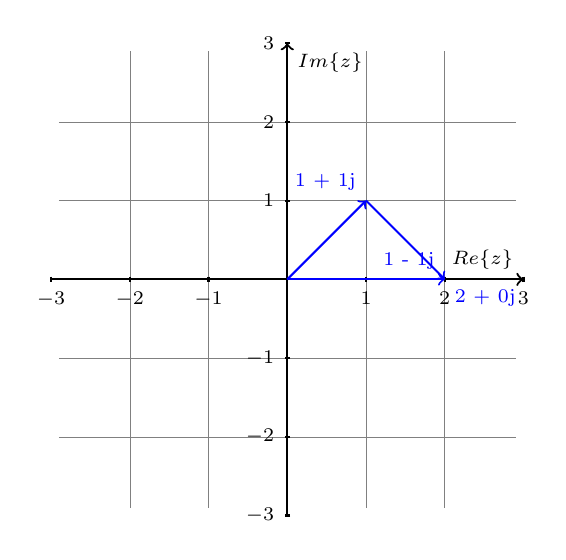
\begin{tikzpicture}
    \begin{scope}[thick,font=\scriptsize]
    \draw[step=1cm,gray,very thin] (-2.9,-2.9) grid (2.9,2.9);
    \draw [->] (-3,0) -- (3,0) node [above left]  {$Re\{z\}$};
    \draw [->] (0,-3) -- (0,3) node [below right] {$Im\{z\}$};

    \foreach \x in {-3, -2, -1, 1, 2, 3}
       \draw (\x cm,1pt) -- (\x cm,-1pt) node[anchor=north] {$\x$};
    \foreach \y in {-3, -2, -1, 1, 2, 3}
        \draw (1pt,\y cm) -- (-1pt,\y cm) node[anchor=east] {$\y$};


    \draw [line width=0.25mm, blue, ->] (0,0) -- (1,1) node [above left] {1 + 1j};
    \draw [line width=0.25mm, blue, ->] (1,1) -- (2,0) node [above left] {1 - 1j};
    \draw [line width=0.25mm, blue, ->] (0,0) -- (2,0) node [below right] {2 + 0j};
    \end{scope}
\end{tikzpicture}

}

\qitem Recall that Euler's Formula states that $e^{j\theta} = \cos(\theta) + j\sin(\theta)$.

\textbf{Using Euler's identity, show the following identities}, which show that sinusoids are sums of complex exponentials:

\begin{align*}
    \cos(\theta) = \frac{e^{j\theta} + e^{-j\theta}}{2} \\
    \sin(\theta) = \frac{e^{j\theta} - e^{-j\theta}}{2j}
\end{align*}

\sol{

  $$e^{j\theta} = \cos(\theta) + j\sin(\theta)$$

  Note that $e^{j\theta}$ has the complex conjugate $e^{-j\theta}$, which means:

  $$e^{-j\theta} = \cos(\theta) - j\sin(\theta)$$
  $$e^{j\theta} +  e^{-j\theta} = \cos(\theta) + j\sin(\theta) + \cos(\theta) - j\sin(\theta)$$
  $$e^{j\theta} +  e^{-j\theta} = 2\cos(\theta)$$
  $$cos(\theta) = \frac{1}{2}(e^{j\theta} +  e^{-j\theta})$$

  We can also notice that this is true because $cos$ is an even function and $sin$ is an odd function, which gives the properties
  $cos(-\theta) = cos(\theta)$ and $sin(-\theta) = -sin(\theta)$.

  A similar approach can be used to find $sin(\theta)$:

  \begin{align*}
    e^{j\theta} - e^{-j\theta} &= cos(\theta) + jsin(\theta) - (cos(\theta) - jsin(\theta)) \\
    &= 2jsin(\theta) \\
    \implies sin(\theta) &= \frac{e^{j\theta} - e^{-j\theta}}{2j}
  \end{align*}

}

\end{enumerate}

\newpage

\end{qunlist}

\end{document}
